\documentclass{article}
\usepackage{graphicx}
\usepackage{setspace}
\usepackage{hyperref}
\setstretch{1.5}

\title{Progetto di Fondamenti di Intelligenza Artificiale\\SignHelper: Parlare a gesti (riconoscimento del linguaggio dei segni americano)}
\author{Vito Gerardo Piegari\\Matricola: 0512110333}
\date{}

\begin{document}

\maketitle
\begin{center}
  
\includegraphics[width=0.5\textwidth]{unisa_logo.png}
\end{center}

\newpage

\renewcommand{\contentsname}{Indice}
\tableofcontents

\newpage

\section{Introduzione}
L'atto di comunicare attraverso il linguaggio dei segni, inizialmente appreso dai bambini come un passatempo, si evolve ben presto in una competenza fondamentale che, una volta acquisite le nozioni basilari dell'alfabeto gestuale, consente una comunicazione agevole senza ricorrere alla verbalizzazione.\\
Tuttavia, vi sono situazioni in cui il linguaggio dei segni non costituisce un mero passatempo ludico, bensì una necessità imprescindibile, specialmente quando sorgono difficoltà nel parlare o sono presenti condizioni di disabilità.\\
Comprendere e comunicare con il linguaggio dei segni, diventa oltre ad un modo divertente di comunicare, anche un modo per favorire l'\textbf{inclusione} nella vita di tutti i giorni di persone che non riescono a comunicare vocalmente.\\
Nonostante la comprensione del linguaggio dei segni sia relativamente facile per le persone, non si può dire lo stesso per i computer, quindi, questo progetto ha come obiettivo quello di implementare una "semplice" intelligenza artificiale in grado di comprendere brevi parole comunicate con il linguaggio dei segni.\\
Il progetto è disponibile su GitHub al seguente link: https://github.com/veetaw/fia

\newpage
\section{Definizione del problema}

\subsection{Obiettivi}
Lo scopo del progetto consiste nel creare una intelligenza artificiale in grado di capire il linguaggio dei segni.

\subsection{Specifica PEAS}
La specifica Peas (Performance Environment Actuators and Sensors) è il primo e fondamentale passo per la formalizzazione del nostro problema attraverso un modello capace di descriverne velocemente le caratteristiche fondamentali.
Nel caso di questo progetto, la specifica PEAS dell'ambiente operativo è la seguente:
\begin{itemize}
  \item \textbf{Performance:} La misura di prestazione del sistema si basa sulla capacità dell'agente nella corretta identificazione della singola lettera nell'alfabeto dei segni.
  \item \textbf{Environment:} L'ambiente dell'agente è la foto della mano inviata al classificatore
  \item \textbf{Actuators:} Gli attuatori consistono in un sistema di traduzione della foto ricevuta
  \item \textbf{Sensors:} Il sensore è il sistema di ricezione della foto della mano.
\end{itemize}

\subsection{Caratteristiche dell'ambiente}
Dopo aver definito il modello PEAS del nostro problema è fondamentale definirne le caratteristiche dell'ambiente in cui opererà:
\begin{itemize}
    \item L'ambiente è \textbf{completamente osservabile}, poichè l'agente riceve sempre lo stato completo di esso dato che l'input è una immagine,
    \item L'ambiente è \textbf{stocastico} poichè l'interpretazione dell'immagine corrente non influenza quella successiva,
    \item L'ambiente è \textbf{statico} poichè l'agente analizza dei fotogrammi che non possono variare mentre l'agente sta deliberando,
    \item L'ambiente è \textbf{singolo} poichè ammette un solo agente,
    \item L'ambiente è \textbf{discreto} poichè c'è un numero possibile di azioni finito (le lettere dell'alfabeto trattato sono 24\footnote{Ovviamente le lettere dell'alfabeto americano sono 26, ma il dataset utilizzato ha evitato le lettere Z e J poichè richiedono movimenti con la mano}).
\end{itemize}

\newpage

\section{Dataset}
Il dataset che è stato scelto di utilizzare si chiama sign-language-mnist, è disponibile su kaggle al seguente \href{https://www.kaggle.com/datasets/datamunge/sign-language-mnist}{link}.\\
Questo dataset è ispirato al celebre dataset MNIST che tratta di cifre e lettere scritte a mano, ne condivide alcune caratteristiche come la presenza di label e di immagini di dimensione 28x28.
\subsection{Struttura}
Il dataset è fornito con una serie di immagini suddivise per classi, che indicano la lettera associata al gesto.\\
Il dataset è provvisto soltanto di 24 delle 26 lettere poichè le lettere Z e J richiedono movimenti della mano.
\begin{center}
    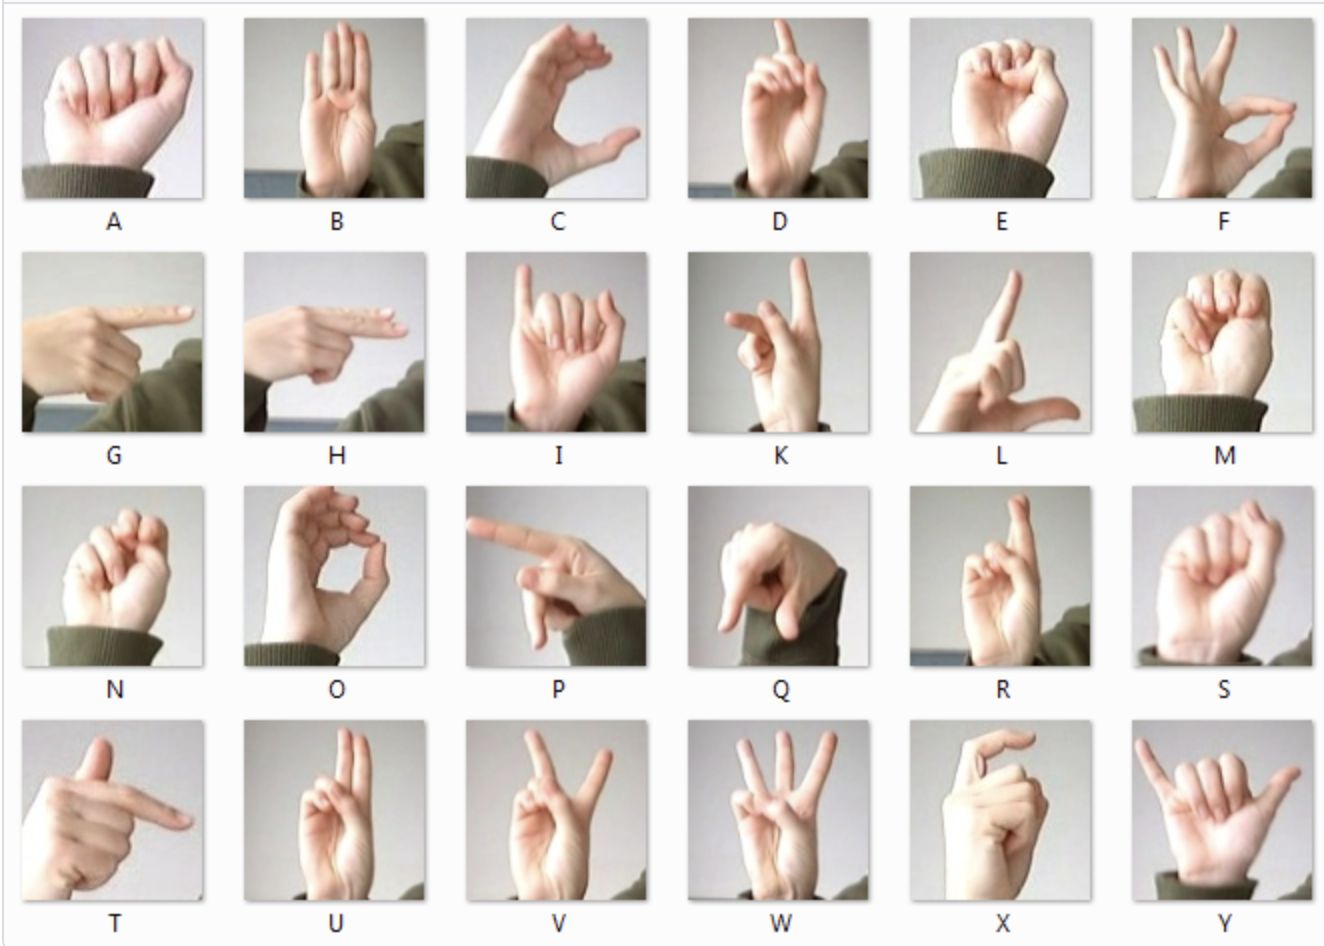
\includegraphics[width=0.9\textwidth]{immagini.png}
\end{center}

\subsection{Bilanciamento del dataset}
Da una prima analisi si evince che il dataset di allenamento è leggermente sbilanciato, quindi sono state necessarie operazioni di data cleaning per evitare possibili problemi di overfitting causati dalla maggiore presenza di alcune classi rispetto ad altre.
\begin{center}
    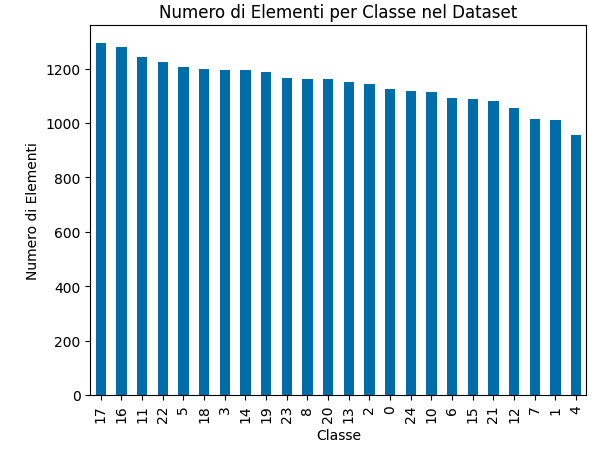
\includegraphics[width=0.9\textwidth]{dataset.png}
\end{center}
In questo caso è stato scelto di prendere la classe con meno elementi nel dataset e fare undersampling sulle altre classi andando a rimuovere i dati in eccesso per livellare tutte le classi sullo stesso numero di elementi.
\begin{center}
    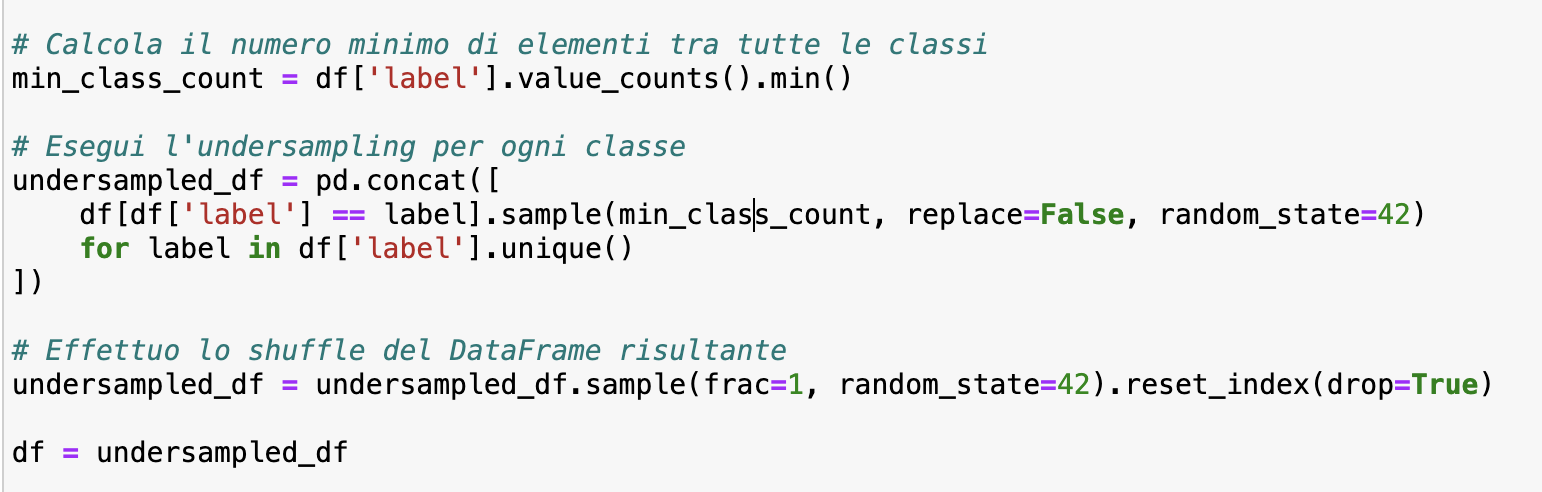
\includegraphics[width=0.9\textwidth]{codice_undersampling.png}
\end{center}
A qusto punto l'operazione di bilanciamento è conclusa poichè il dataset, come si evince dal prossimo grafico, risulta bilanciato.
\begin{center}
    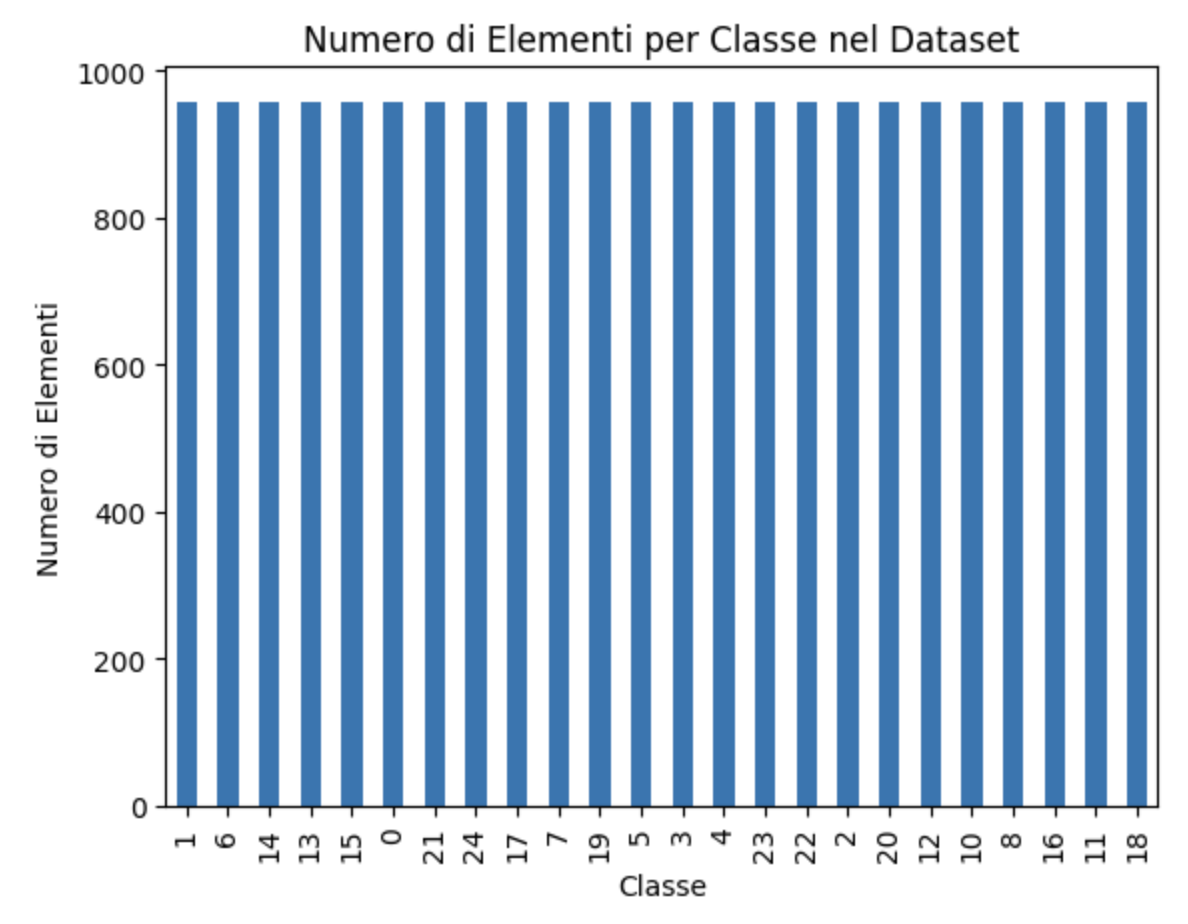
\includegraphics[width=0.9\textwidth]{dataset_bilanciato.png}
\end{center}

\subsection{Ulteriori operazioni sui dati}
Dato che il nostro dataset è un csv in cui ogni riga è composta da una label e 784 celle successive, è stato necessario trasformare il vettore dei pixel dell'immagine in una matrice 28x28.
\begin{center}
    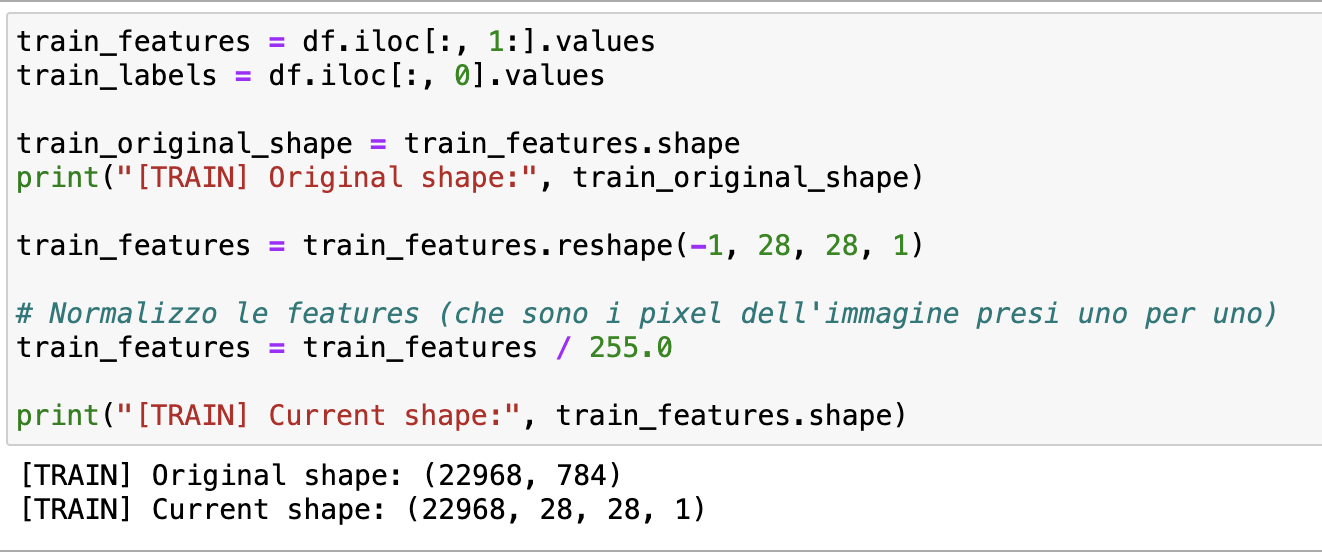
\includegraphics[width=0.9\textwidth]{shape.png}
\end{center}
Notiamo come il risultato dell'operazione di reshaping sia, appunto una matrice 28x28 con un solo canale colore (dato che le immagini sono in scala di grigi).


\newpage
\section{Soluzione proposta}
La soluzione proposta è un modello di Machine Learning in grado di riconoscere la lettera associata al gesto fatto con la mano, passato al modello come foto.
\subsection{Modello}
Il modello scelto è una CNN (Convolutional Neural Network), che ha come obiettivo quello di classificare, tramite varie operazioni, l'immagine ad esso inviata e restituirne la classe di appartenenza (in questo caso la lettera).
\subsection{Composizione CNN (Convolutional Neural Network)}
Nella composizione della rete neurale sono stati utilizzati i seguenti layer:
\begin{itemize}
  \item \textbf{Conv2d} : Questo tipo di layer si occupa dell'operazione di convoluzione, ossia far passare un kernel(filtro) di dimensione 2x2 nell'immagine per iniziare a mappare le caratteristiche dell'immagine. A questo layer è associata la funzione di attivazione ReLU che si occupa di introdurre non linearità
  \item \textbf{MaxPool2d} : Questo tipo di layer non apprende nulla, ma svolge un ruolo importante nella feature extraction, infatti verrà fatto passare un kernel 2x2 nell'immagine e verrà preso il pixel con il valore pià alto. Questo tipo di operazione serve a togliere ancora di più linearità nell'immagine e di conseguenza andare a limitate situazioni di overfitting.
  \item \textbf{Dropout} : Questo tipo di layer ha come compito quello di disconnettere casualmente un certo numero di neuroni, impedendo loro di contribuire all'output in quel passaggio. I layer di dropout sono utili a limitare l'overfitting.
  \item \textbf{Flatten} : Questo layer si occupa di convertire l'output della convoluzione in un vettore monodimensionale. Questo permette di passare dalla rappresentazione spaziale delle caratteristiche estratte dai filtri convoluzionali a una rappresentazione unidimensionale che può essere utilizzata dai layer densamente connessi.
  \item \textbf{Dense} : Questo tipo di layer, anche chiamato layer densamente connesso poichè ogni nodo (neurone) è connesso con tutti i nodi del layer precedente, utilizzato con funzione di attivazione softmax si occupa di creare una distribuzione di probabilità su tutte le classi di output, quindi è il responsabile della predizione del risultato.
\end{itemize}
Dopo un'analisi iterativa della rete neurale, provando più combinazioni di layer, è stato notato che il miglior risultato è ottenuto con la seguente composizione:
\begin{center}
    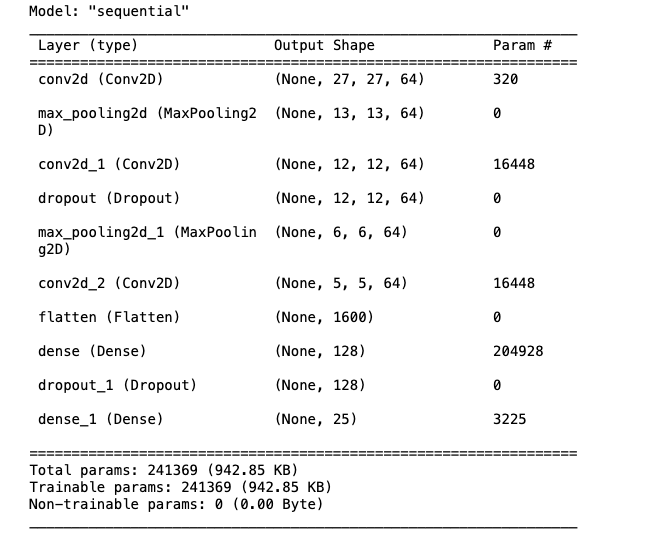
\includegraphics[width=0.9\textwidth]{layers.png}
\end{center}
Inoltre, è stato scelto di usare un kernel di dimensione 2x2 per i layer di convoluzione, poichè:
\begin{itemize}
    \item Impostando un kernel per il layer convoluzionale 2x2 ho una accuracy del 99\% sul dataset di TRAIN dopo 1 epoca, su quello di test 90%
    \item Impostando un kernel per il layer convoluzionale 3x3 ho una accuracy del 95\% sul dataset di TRAIN dopo 1 epoca, su quello di test 89%
\end{itemize}
Creata la rete neurale, viene compilato il modello con le API messe a disposizione da Tensorflow, utilizzando i seguenti parametri:
\begin{itemize}
    \item \textbf{Optimizer}: \textit{Adam}, un algoritmo di ottimizzazione che adatta dinamicamente i tassi di apprendimento durante l'allenamento.
    \item \textbf{Funzione di perdita}: \textit{sparse\_categorical\_crossentropy}, una loss function utilizzata per problemi di classificazione in cui le etichette sono intere, come nel caso studiato.
    \item \textbf{Metriche}: è stato deciso di usare l'\textit{accuracy} come metrica da monitorare durante l'allenamento del modello, ricordando che l'accuratezza è calcolata come $Accuracy_{modello} = \frac{(TP + TN)}{(TP + TN + FP + FN)}$.
\end{itemize}

\subsection{Miglioramento del modello}
Dopo i primi test il modello risultava funzionare molto bene sui dati di testing e di training, ma dava problemi con dati nuovi, quindi vi era presenza di overfitting. Questo problema è stato risolto aggiungendo un layer di Dropout e prendendo dei dati dal dataset di training e usandoli come dati di validazione durante l'addestramento del modello.\\
Queste operazioni hanno portato ad una significativa diminuizione dell'accuratezza sui dati di training al pari di numero di epoche, ma ad un importante aumento dell'accuratezza sui dati di test. \\
Incrementando, poi, il numero di epoche a 10 è stata raggiunta una accuratezza sul dataset di training dell'80\% (contro la precedente 95\%), e dell'95\% sul dataset di testing (contro la precedente 89\%).
\begin{center}
    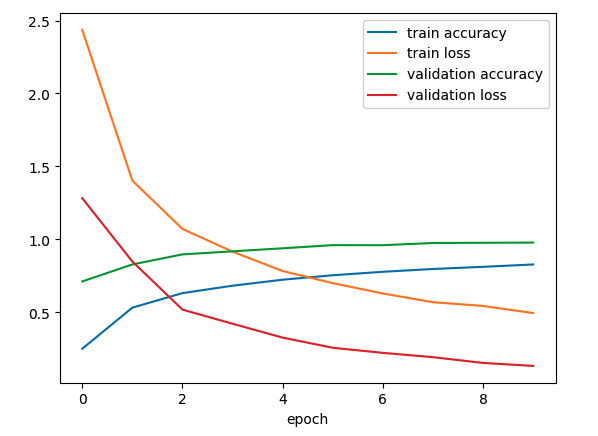
\includegraphics[width=0.9\textwidth]{accuracy.png}
\end{center}
Il modello risultava a questo punto significamente migliore di quello iniziale, ma continuava ad avere problemi con foto esterne, scattate in condizioni diverse da quelle che aveva visto durante il training.\\
Per risolvere questo problema sono state adottate due strategie parallele: effettuare data augmentation sul dataset di training e maggiore preprocessing sulle immagini per valorizzarne i dettagli utili.
\subsubsection{Data augmentation}
Considerando che le foto scattate da un potenziale utente non hanno sempre un perfetto sfondo bianco dietro o che la mano non si trova nella perfetta angolazione si è deciso di effettuare un'operazione di data augmentation sul dataset. Questo tipo di operazione serve a generare nuova conoscenza per il modello, basandosi sulle immagini già presenti e effettuando sopra di esse operazioni quali rotazione, zoom, shift, specchiamento, etc... \\
Nel caso di questo modello è stato scelto di effettuare le seguenti operazioni:
\begin{itemize}
    \item \textbf{Rotazione} nel range di [-10, +10] gradi. Questo range è stato scelto poichè una rotazione eccessiva avrebbe potuto confondere il modello,
    \item \textbf{Zoom} nel range di [-0.1, +0.1],
    \item \textbf{Shift} sia in altezza che in larghezza per allenare il modello su foto in cui la mano potrebbe essere leggermente decentrata.
\end{itemize}
\subsubsection{Preprocessing dell'immagine}
Questo tipo di operazione è stata messa in atto poichè lo sfondo dietro la foto del gesto fatto con la mano potrebbe confondere il modello. Durante lo sviluppo di questa parte del progetto sono state testate diverse tecniche per massimizzare i dettagli della mano, come aumentare la luminosità o il contrasto dell'immagine, alcune di esse portavano a benefici, altre peggioravano le predizioni del modello.\\
L'equilibrio è stato raggiunto semplicemente trasformando l'immagine in scala di grigi, rimuovendo lo sfondo alla mano attraverso la libreria \textit{rembg} e incollandola su uno sfondo grigio, per poi ridimensionare l'immagine in 28x28.
\begin{center}
    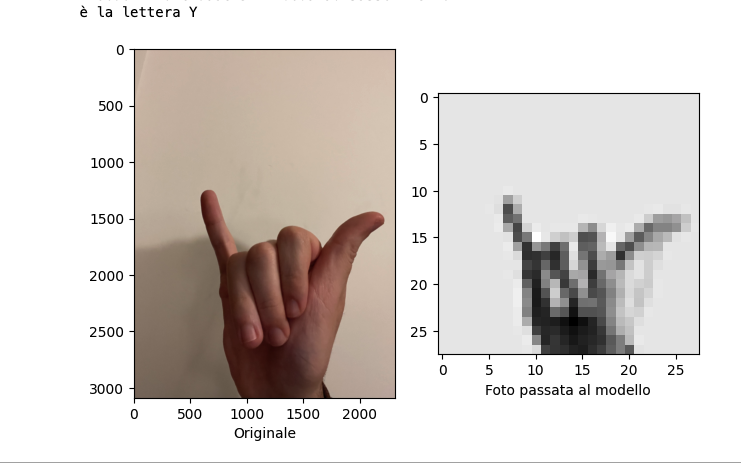
\includegraphics[width=0.9\textwidth]{preprocess.png}
\end{center}
A questo punto per migliorare ancora di più il modello sono state effettuate alcune prove come quella di diminuire la lunghezza del batch da 32 a 16, che ha contribuito al risultato finale del modello.\\
\subsection{Riepilogo}
I dati di accuracy e loss finali sono stati i seguenti (il modello è stato allenato per 10 epoche):
\begin{center}
    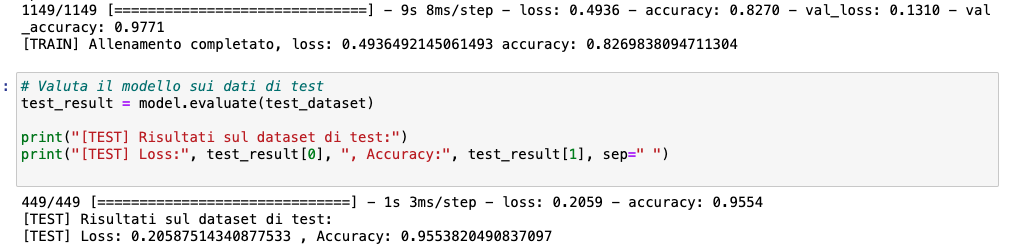
\includegraphics[width=0.9\textwidth]{final_acc.png}
\end{center}

\newpage
\section{Conclusioni}
Questo progetto è stato sviluppato come approfondimento per il corso, il modello non è perfetto, ma si è cercato di ottenere il massimo sfruttando le conoscenze apprese durante il corso e su internet, oltre che effettuando una sperimentazione continua per cercare di migliorare il risultato finale.
 
\subsection{Sviluppi futuri}
Questo modello non è facilmente utilizzabile da utenti comuni, per questo motivo una possibile modifica da fare sarebbe quella di implementare una applicazione user-friendly in modo da rendere utilizzabile il sistema a tutti.\\
Un'altra possibile implementazione futura sarebbe quella di avere un sistema che supporta il linguaggio dei segni "completo", quindi in grado di funzionare come una specie di t9, completando le parole e quindi velocizzando la comunicazione. Un sistema di questo tipo potrebbe essere ancora più utile integrato in sistemi di videocall come Whatsapp, Teams, Zoom, etc...

\end{document}
